\documentclass[letterpaper,10pt,draftclsnofoot,onecolumn,compsoc,titlepage]{IEEEtran}

\usepackage{graphicx}
\usepackage{amssymb}
\usepackage{amsmath}
\usepackage{amsthm}
\usepackage{alltt}
\usepackage{float}
\usepackage{color}
\usepackage{url}
\usepackage{enumitem}
\usepackage{pstricks, pst-node}
\usepackage{geometry}

\graphicspath{ {./figures/} }

\geometry{margin = .75in}

\usepackage{hyperref}

\newcommand*{\signature}[1]{%
	\par\noindent\makebox[3.5in]{\hrulefill} \hfill\makebox[3.0in]{\hrulefill}%
	\par\noindent\makebox[3.5in][l]{#1}	    \hfill\makebox[3.0in][l]{Date}%
}%

\def\name{Kevin Stine, Courtney Bonn, Maxwell Dimm}
\def\team{A Connection App for a Local Non-Profit Organization}

\hypersetup{
	colorlinks = true,
	urlcolor = black,
	linkcolor = black,
	pdfauthor = {\name},
	pdftitle = {CS461 Requirements},
	pdfsubject = {CS461 Requirements},
	pdfpagemode = UseNone
}

\begin{document}
	\title{\huge \team \\ Requirements Document \\ CS 461 Fall 2016}
	\author{\large \name}

	\maketitle
		\begin{abstract}The purpose of this project is to produce an iOS/Android application for Calvary Chapel of Corvallis that will allow members to access a plethora of information all in one localized space.
		The Church's current website doesn't provide an interface where current members of the church can very quickly access important information such as events, bulletins, and messages from the service.
		The desired application will be simple enough for anyone to use while providing back end access for staff to easily upload new information to the app.
		The priorities lie in maximizing the usability of the app and providing bulletin, schedule, video, and donation functionality.
		We will work with the existing Calvary Chapel web development team to create a product that is seamlessly integrated with their already existing network.
		\end{abstract}

	\clearpage
	
	\tableofcontents
	
	\clearpage

	\section{Introduction}
	\subsection{Purpose}
	The purpose of this document is to list, in detail, all of the requirements intended for our project.
	Additionally, there will be an overall description of the project, explaining the different aspects of the application in which we are building.
	This document is intended for the client team at Calvary Chapel of Corvallis, as well as the teachers and teachers assistants for our class.

	\subsection{Scope}
	At the completion of this project, the software product to be produced is called The Calvary Chapel of Corvallis App (placeholder for official name).
	This application will provide a portion of the information already available on the church website in a mobile-friendly application.
	The application will not be an exact replica of the website, but rather a combination of certain sections that are used heavily by current members of the church.
	The main goal of the application is to offer a space for the active members of the church to stay current with events, messages, and the e-bulletin.
	It will benefit the church members in a different way than their current website, because the application will allow them to have all of the necessary information saved on their smartphone, rather than opening a new browser each time they need to access the website.
	In order to ensure this application is available to all members, the application will be offered for both iOS and Android users.

	\subsection{Definitions, acronyms, and abbreviations}

	\begin{enumerate}
		\item \textbf{Android:} A mobile operating system developed by Google, based on the Linux Kernel and designed primarily for touchscreen mobile devices.
		\item \textbf{iOS:} A mobile operating system created and developed by Apple Inc. exclusively for Apple's hardware.
		\item \textbf{App:} A software application designed to run on mobile devices such as smartphones or tablet computers.
		\item \textbf{App Store:} Apple's digital distribution platform for mobile software applications.
		\item \textbf{Google Play Store:} Google's digital distribution platform for mobile software applications.
	\end{enumerate}

	\subsection{References}
	\begin{enumerate}
		\item \textbf{iOS Design Guidelines:} https://developers.apple.com/design/
		\item \textbf{iOS Human Interface Guidelines} https://developers.apple.com/ios/human-interface-guidelines/
		\item \textbf{Android Design Guidelines:} https://developer.android.com/design/index.html
	\end{enumerate}

	\subsection{Overview}
	 The rest of this document contains information on what features are expected to be in the app and descriptions of those features.

	\section{Overall description}
	\subsection{Product perspective}
	The Calvary Chapel of Corvallis App is a mobile application that will be optimal for both iOS and Android users.
	This application will incorporate information that is present on the desktop website that is currently available.
	The information that will be shared between the mobile application and the desktop website includes calendar events, messages, and the e-bulletin.

	\subsubsection{System interfaces}
	Each user will be able to use this application on iOS and Android smartphones.
	To use the application, the user will have to download the application directly to their smartphone from the App Store and/or the Google Play Store.
	Once downloaded to the user's phone, there will be no additional software needed to use the application.

	\subsubsection{User interfaces}
	The interface should be very simple and easy to understand.
	There should not be more than five to six clickable options per page.
	Also the users should be able to find any available information on the app within three clicks or taps.
	The menu will either be a standard navigation bar at the top, or a clickable icon menu whichever proves more usable after testing.

	The Calvary Chapel of Corvallis App will adhere to the design guidelines specified by both Apple and Google.
	The iOS and Android version of the app will be built with adaptability in mind.
	As iPhones and Android phones have various screen sizes, our app will scale appropriately on all screen sizes.

	The app will have the various categories which the user can interact with:
	\begin{enumerate}
		\item \textbf{Announcements:} The user should be able to view all the recent announcements.
		\item \textbf{Events:} The user should be able to view a calendar or list of events that are upcoming as well as past events.
		\item \textbf{Donations:} The user should be able to donate to the church quickly and securely.
		\item \textbf{Sermons:} The user should be able to view and/or listen to the most recent sermons.
	\end{enumerate}



	The iOS version of the app will follow these three primary themes:
	\begin{enumerate}
		\item \textbf{Clarity:} Throughout the system, text is legible at every size, icons are precise and lucid, adornments are subtle and appropriate, and a sharpened focus on functionality motivates the design.
		Negative space, color, fonts, graphics, and interface elements subtly highlight important content and convey interactivity.
		\item \textbf{Deference:} Fluid motion and a crisp, beautiful interface help people understand and interact with content while never competing with it.
		Content typically fills the entire screen, while translucency and blurring often hint at more.
		Minimal use of bezels, gradients, and drop shadows keep the interface light and airy, while ensuring that content is paramount.
		\item \textbf{Depth:} Distinct visual layers and realistic motion convey hierarchy, impart vitality, and facilitate understanding.
		Touch and discoverability heighten delight and enable access to functionality and additional content without losing context.
		Transitions provide a sense of depth as you navigate through content.
	\end{enumerate}

	\subsubsection{Hardware interfaces}
	Apple iPhones and Android smartphones will be the devices that are supported by the application.

	\subsubsection{Software interfaces}
	We will be incorporating the church's current system for keeping track of their calendar into the new application.
	The software used by the church is called Church Community Builder.
	We will use the software's API to connect the existing calendar to the mobile application, which will prevent the church staff from having to update two different calendars.

	\subsubsection{Communications interfaces}
	Within the app there will be a page that allows users to connect to the churches existing social media.
	There should also be the ability to send notices or messages to the churches administration.

	\subsubsection{Memory}
	The app should not take up more than 500 Mb of storage.
	If time allows as well we aim to give users the ability to take down notes within the app.

	\subsubsection{Operations}
	The app should be able to display pdf or text messages of their bulletin and schedule.
	It should also have audio or possibly video support for their past sermons.
	It should also take input from the user when taking notes or in the giving portions of the app.

	\subsection{Product functions}
	The product or app we are making is intended to be a next step for the members to connect with the church after visiting their website.
	It is not functioning the same way as the website.
	The website is meant as an introduction to the church, the app is the connection that will be made after members have connected.
	The app itself will have a couple functions but the general idea is that when people who call Calvary Corvallis their home want to access information about the church, they should go to this app to find it.
	The apps four primary functions will be an announcements page, the church schedule or calendar, a place to watch/listen to the sermons, and the ability to give to the church.

	\subsection{User characteristics}
	The intended user is the average, every day person who attends Calvary Corvallis Church.
	The application can be used by some with little to extensive education.
	It will be simple enough that people who are not as experienced with smartphones will still be able to use and understand the application.
	Technical expertise will only be required for the team of people who will be monitoring and updating the application.
	
	We will have two phases of testing for this project. 
	The first phase will take place during the initial design of the app. 
	This phase will be used to test the design before we begin coding.
	We will then use the feedback from test users to edit the design.
	
	The second phase of testing will take place after the alpha level release of the app. 
	During this phase, we will pick a minimum of ten different people who have varying backgrounds in technical experiences. 
	These people will be asked to test the application, by performing a number of tasks that are designed to test the simplicity and functionality of the app. 
	These tasks will include: 
	\begin{enumerate}
		\item{Download the application}
		\item{Find and view the calendar}
		\item{Find and view the announcements}
		\item{Listen to a recent sermon}
		\item{Find the donation page and successfully donate to the church}
		\item{Find and read the recent bulletin}
		\item{Find and visit the church's social networking sites}
	\end{enumerate}
	If 90\% of test users are able to complete all the assigned tasks, then we will consider the application successful. 
	We will ask for feedback from the users on the simplicity of finding each section of the app and how many clicks it took them to reach a destination.
	Additionally, we will ask for feedback on the basic functionality of the app and whether or not they felt it was easy to navigate and worked as intended.
	
	If more than 10\% of the test users fail the assigned tasks, then we will need to review the design of the application. 
	We will use the feedback from the users and incorporate changes accordingly. 
	After we handle all the necessary changes, we will perform this phase of testing again. 

	\subsection{Constraints}
	The client has requested that the app is simple and does not have an overly complicated color scheme.
	The app needs to also be secure when handling peoples donations, so their information will need to be encrypted.
	The app should also run smoothly on all modern smartphones made in the last 3 to 4 years.
	Also the app should run quickly enough that any information that can be found on the app should be accessible quicker than navigating to their website.

	\subsection{Assumptions and dependencies}
	This project assumes that the application will be accepted by Apple into the official app store.
	If it is not accepted, then there will be additional work needed to ensure the app follows the official Apple guidelines.

	\subsection{Apportioning of requirements}
	Our first task will be to complete a technology review that goes into depth about the already available technology that can assist us with our project. 
	Next, we will create a design document that will detail the design of our project. 
	
	Some of the features of the app that can be further developed over time would be the video support for the sermon. 
	At first we plan to develop to have the audio sermons on the app, but if the church has the video available we can work towards making that available in future versions of the app. 
	There is the possibility to have the ability for members to RSVP or confirm attendance to specific events in future versions of the app as well.
	

	\section{Specific requirements}
	\subsection{External Interfaces}
	The only external interface needed for this app to work properly is a iOS or Android smartphone that has the most up-to-date software.
	No other external interfaces are required for the functionality of the app.

	\subsection{Functions}
	This app should be a relatively simple interface that allows the user to connect with the church's most important functions.
	The functions that will be included are:
	\begin{enumerate}
		\item{Announcements:}
			\begin{itemize}
				\item{Add new announcement}
				\item{Edit or delete an announcement}
				\item{View an announcement}
				\item{View previous announcements}
			\end{itemize}
		\item{Calendar:}
			\begin{itemize}
				\item{View details for an event}
				\item{View previous months}
			\end{itemize}
		\item{Sermons:}
			\begin{itemize}
				\item{Upload new sermon}
				\item{Delete/archive a sermon}
				\item{Listen to a sermon}
			\end{itemize}
		\item{Donations:}
			\begin{itemize}
				\item{Donate}
			\end{itemize}
	\end{enumerate}


	\subsection{Performance requirements}
	Any number of users should be able to download the application and have it stored on their phone.
	The app should support all users simultaneously.

	\subsection{Design constraints}
	There are design constraints imposed by Apple guidelines for iOS applications.
	Additionally, the client would like a simple design that makes it easy for non-technical users to navigate the app with little to no help.

	\subsection{Software system attributes}
	\subsubsection{Reliability} The app should operate well under all conditions and be considered reliable enough to be used for any amount of time without failing.
	\subsubsection{Availability} The app should be available at all times, unless there is scheduled maintenance that requires it to be down for a minimal amount of time.
	\subsubsection{Security} Because users will be using personal information for the donations, the app should be considered secure and
	\subsubsection{Maintainability} The app will be simple enough that is is able to be maintained by the existing website development team at Calvary Chapel Corvallis.
	\subsubsection{Portability} The app should be portable as it should run on two different platforms: iOS and Android.

	\begin{figure}[p]
	    \centering
	    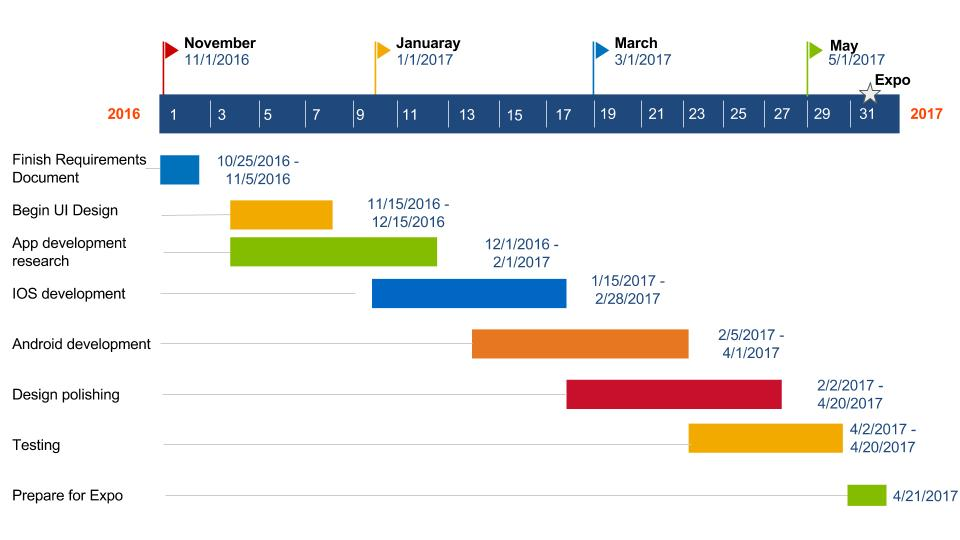
\includegraphics[width=7in, height=6in, natwidth=960, natheight=540]{Gantt.jpg}
	    \caption{Project Timeline}
	\end{figure}

	\clearpage
	
	\section*{Signatures}

	\vspace{1in}
	\signature{Client}
	\vspace{1in}
	\signature{Courtney Bonn}
	\vspace{1in}
	\signature{Kevin Stine}
	\vspace{1in}
	\signature{Maxwell Dimm}

\end{document}
